\documentclass[10pt]{article}
\usepackage[paper=letterpaper,margin=2cm]{geometry}
\usepackage{amsmath}
\usepackage{amssymb}
\usepackage{amsfonts}
\usepackage{newtxtext, newtxmath}
\usepackage{enumitem}
\usepackage{titling}
\usepackage{graphicx}    %  in the preamble
\usepackage{fancyhdr}
\usepackage{subcaption}
\usepackage[colorlinks=true]{hyperref}

\setlength{\droptitle}{-10em}

\fancyhf{}
\fancyhead[L]{MATH 232: Linear Algebra}
\fancyhead[R]{Steven Wong, 301337727}
\renewcommand\headrulewidth{0pt}
\pagestyle{fancy}

\begin{document}

\noindent\makebox[\textwidth][c]{\Large\bfseries Assignment 2}
\normalsize
\begin{enumerate}[leftmargin=\labelsep]
    \item[1A.)] Let $x_1 = \begin{bmatrix} 2 \\ 5 \end{bmatrix} \text{ and } x_2 = \begin{bmatrix} 8 \\ 13 \end{bmatrix}$ be vectors representing a rectangle's terminal points. 
    I have selected to apply a $5$ magnitude stretch in the $x$-direction ($A_1)$, and a reflection about the $y$-axis ($A_2$). These geometric transformations
    can be represented by the following matrices respectively:
    
    \[
        A_1 = 
        \begin{bmatrix}
            5 & 0 \\
            0 & 1
        \end{bmatrix} A_2 =
        \begin{bmatrix}
            -1 & 0 \\
            0 & 1
        \end{bmatrix} 
    \]
    
    Applying our transformation matrices, we get the results in Figure 1 where black is our original rectangle, red is our x-direction stretch, and magenta is our y-axis reflection.

    \item[1B.)] If we let $V$ be the matrix operator $V = \begin{bmatrix} 1 & 0 \\ 3 & 1 \end{bmatrix}$ and $S$ be the matrix operator $S = \begin{bmatrix} 1 & 0 \\ 0 & 5 \end{bmatrix}$, then we can see that the composition of $V$ and $S$ does not commute.
    Let us consider the unit square with corners at $(1, 1), (2, 1), (2, 2), (1, 2)$. Applying the composition of $V$ and $S$ in both orders, Figure 2 shows that the resulting shape depends on the order in which the operations are applied.
    
    \begin{figure}[h]
        % Side by side figures 
        \begin{minipage}[c]{0.48\linewidth}
        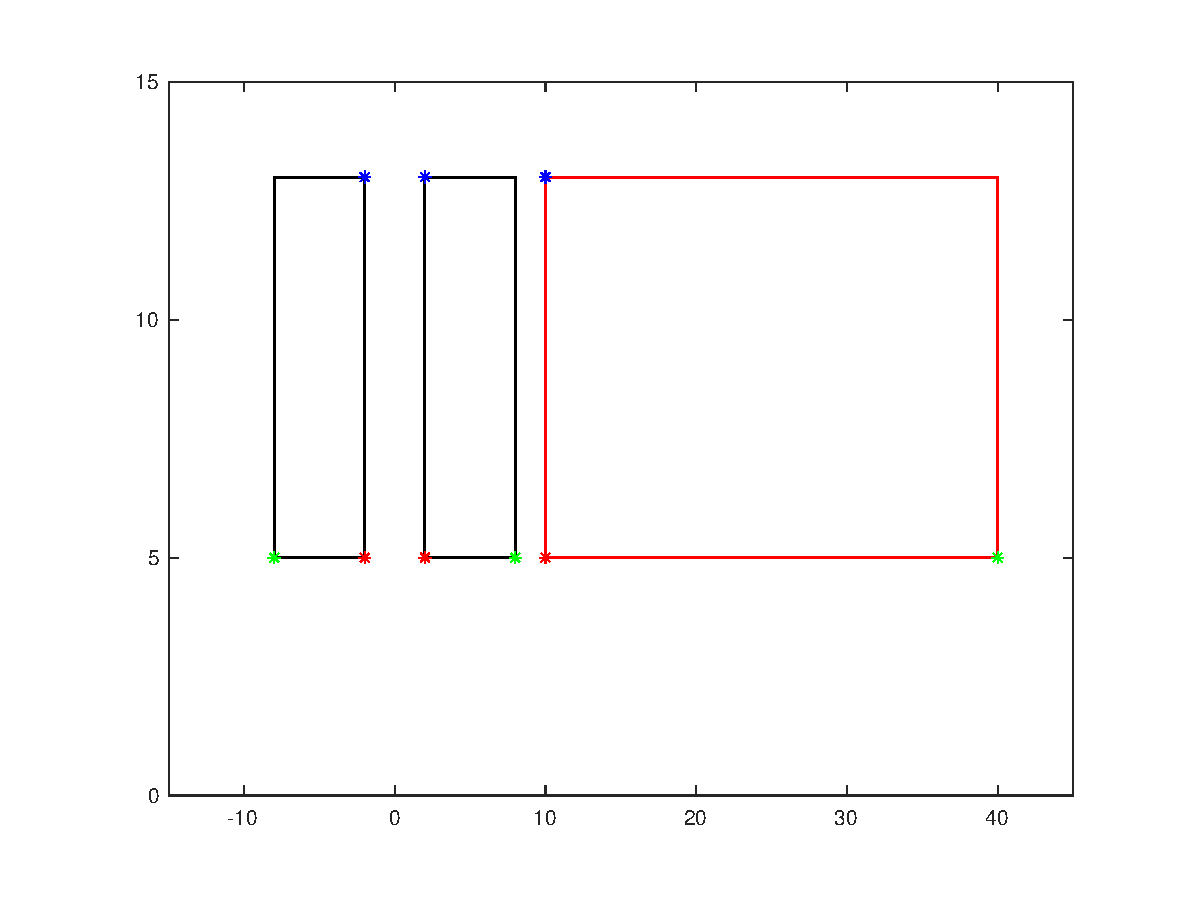
\includegraphics[width=\linewidth]{Figure1.eps}
        \caption{}
        \end{minipage}
        \hfill
        \begin{minipage}[c]{0.48\linewidth}
        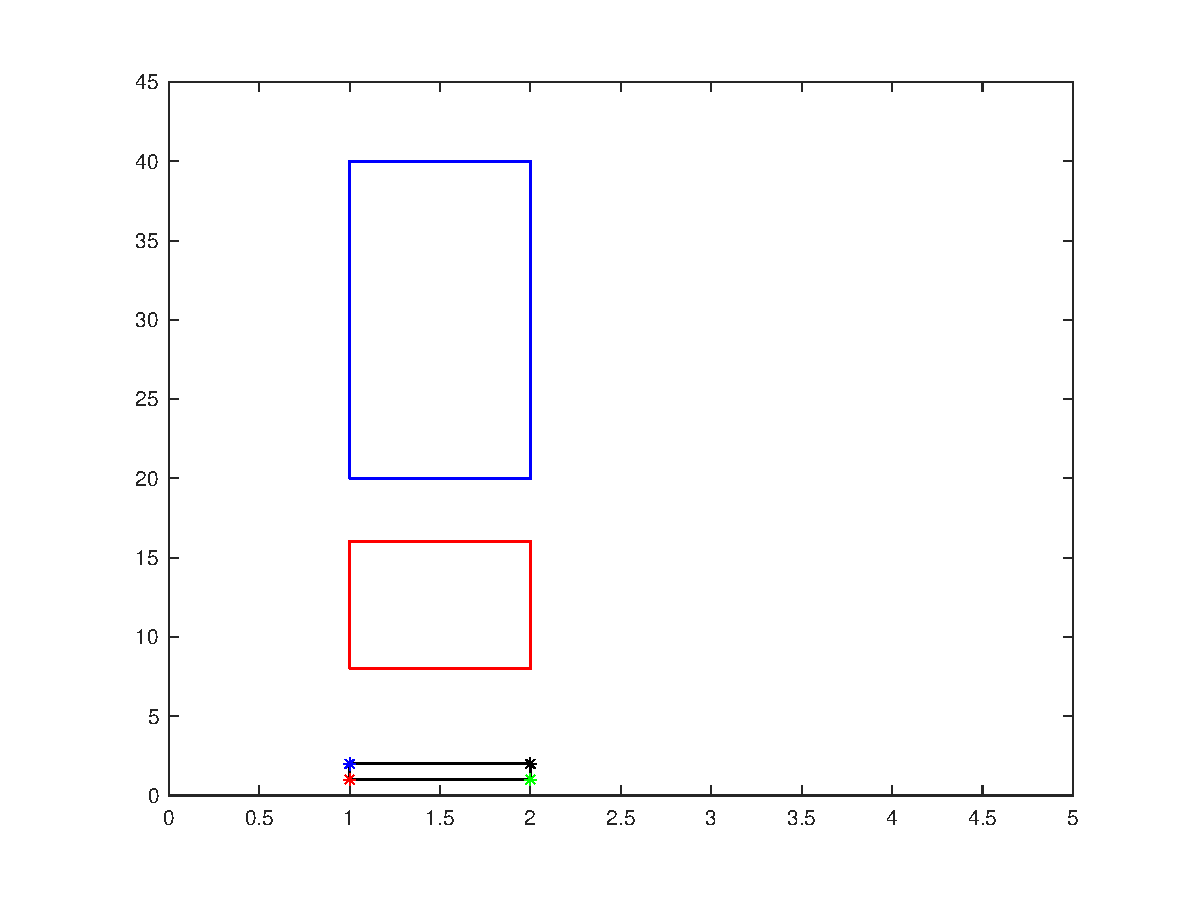
\includegraphics[width=\linewidth]{Figure2.eps}
        \caption{}
        \end{minipage}%
    \end{figure}
    
    This is corroborated by Theorem 3.2.5 of the text which states that the composition of two linear transformation is given by the matrix product of the two transformations. As seen in the following result, the composition of $V$ and $S$ is not equal to the composition of $S$ and $V$. Therefore, 
    it is not commutative. (SHOULD I INCLUDE THE MATRIX COMPLETE RESULT HERE)??
    \begin{equation}
        \begin{bmatrix} 1 & 0 \\ 3 & 1 \end{bmatrix} \begin{bmatrix} 1 & 0 \\ 0 & 5 \end{bmatrix} \neq \begin{bmatrix} 1 & 0 \\ 0 & 5 \end{bmatrix} \begin{bmatrix} 1 & 0 \\ 3 & 1 \end{bmatrix}
    \end{equation}


    \item[2)] To transform the black rectangle into the red rectangle, we need to apply a rotation $R$ of 180 degrees followed by a 
    horizontal stretch $S$. Taking the composition of these two transformations, we obtain the following transformation matrix $A$:

    \[ \text{A: } [R \cdot S] = \begin{bmatrix}
        cos(\pi) & -sin(\pi) \\
        sin(\pi) & cos(\pi)
    \end{bmatrix} \begin{bmatrix}
        2 & 0 \\
        0 & 3.5
    \end{bmatrix} = 
    \begin{bmatrix}
        -2 & 0 \\
        0 & -3.5
    \end{bmatrix} \]

    
\end{enumerate}
\end{document}